% the code below specifies where the figures are stored
\ifpdf
    \graphicspath{{backmatter/figures/PNG/}{backmatter/figures/PDF/}{backmatter/figures/}}
\else
    \graphicspath{{backmatter/figures/EPS/}{backmatter/figures/}}
\fi


\begin{appendices}
\chapter{Data Cleaning}
    \label{sec:dc_appen}
Each data cleaning cut is associated with a bit in a 64-bit binary value called
the data cleaning word or data cleaning mask.
The cuts that each event passes or fails is tracked by its data cleaning mask.
For the solar analyses all events are required to pass all cuts
given by the data cleaning mask \texttt{0xFB0000017FFE}.
This corresponds to the following data cleaning cuts:
    \textbf{Zero Zero Cut},
    \textbf{Crate Isotropy Cut},
    \textbf{FTS Cut},
    \textbf{Flahser Geo Cut},
    \textbf{ITC Time Spread Cut},
    \textbf{Junk Cut},
    \textbf{Muon Tag},
    \textbf{Neck Cut},
    \textbf{Owl Cut},
    \textbf{QCluster Cut},
    \textbf{QvNhit Cut},
    \textbf{QvT Cut},
    \textbf{Ring Of Fire Cut},
    \textbf{Two-Pass Muon Follower, Short},
    \textbf{Polling Cut},
    \textbf{Retrigger Cut},
    \textbf{Two-Pass Burst Cut},
    \textbf{Missed Muon Follower Cut},
    \textbf{Missing CAEN Data Cut},
    \textbf{Ped Cut},
    \textbf{Atmospheric Cut}.
Of those cuts I'll detail here the motivation behind and evaluation of the
cuts that I developed, the cuts that I did not directly develop are described in~\citep{dc_document}.

\section{Ped Cut}
During normal detector operations there are a few trigger calibration
tests that are periodically ran.
These tests use the PEDESTAL signal to inject a certain amount of fake hits
into the detector, and events with those hits are inspected to evaluate the efficiency and
quality of the trigger response.
It's very important that these events are clearly identified and removed from the
dataset so that the fake PEDESTAL hits are not confused for a real signal.
Additionally, the trigger calibration processes usually include changing settings
related to the PEDESTAL signal on the FEC, there's reason to believe these sort
of changes can introduce noise to the front-end.
So an aggressive approach of cutting all events that are within one second of
a pedestal event is used.
This not only cuts events but introduces a dead time into the dataset,
this deadtime is subtracted from the overall livetime.

\section{Missed Muon Follower Cut}
The missed muon follower cut was a data cleaning cut used in SNO, but I adapted
it for SNO+.
In SNO it was very important to identify and cut neutrons that follow
after a cosmic muon event, those neutrons could fake
a neutral current solar neutrino event.
In SNO+ this is not as much a problem because neutron captures in water will
primarily produce a $2.2$\,MeV gamma, which is below the analysis threshold for
solar neutrinos.
However, there does exist events in the dataset which are observed to follow
after high-nhit, events. The origin of these events is not well understood, they
could likely be instrumental, or from  spallation products within the detector.
Since solar neutrino events are not expected to have any time correlations
with other events in the detector, a cut can be placed on the time between
events with relatively little sacrifice.\\

The cut considers three values, an initial and a follower event nhit, $N_{1}$
and $N_{2}$, and a time difference between the two events $\Delta t$;
a threshold is placed on each of these three values, and any pairs of events that cross
each threshold are cut and so is all other events that fall within the threshold
time window.
To evaluate the cut optimal cut criteria for $N_{1}$, $N_{2}$ and $\Delta_{t}$
two different values are considered.
The first is the probability that an event of nhit greater than $N_{2}$ will occur within a time
window $\Delta t$ after an event of nhit greater than $N_{1}$.
This values is called the follower probability, $P_{F}(N_{1}, N_{2}, \Delta t)$.
The second values is the probability that an event of nhit $N$ will occur
within a time window $\Delta t$ that is chosen randomly, this value
is called accidental probability or random coincidence probability, $P_{R}(N, \Delta t)$.
Under the assumption that there is no time correlation with non-background
events the probability of this cut sacrificing a signal event is
\begin{equation}
    \mathrm{Sacrifice} = P_{R}(N_{1},\Delta t)P_{S}(N_{2}) + P_{R}(N_{2}, \Delta t)P_{S}(N_{1})\text{,}
\end{equation}
where $P_{S}(N)$ is the probability for a signal event to have an nhit above
$N$.

\begin{figure}[htbp]
    \centering
    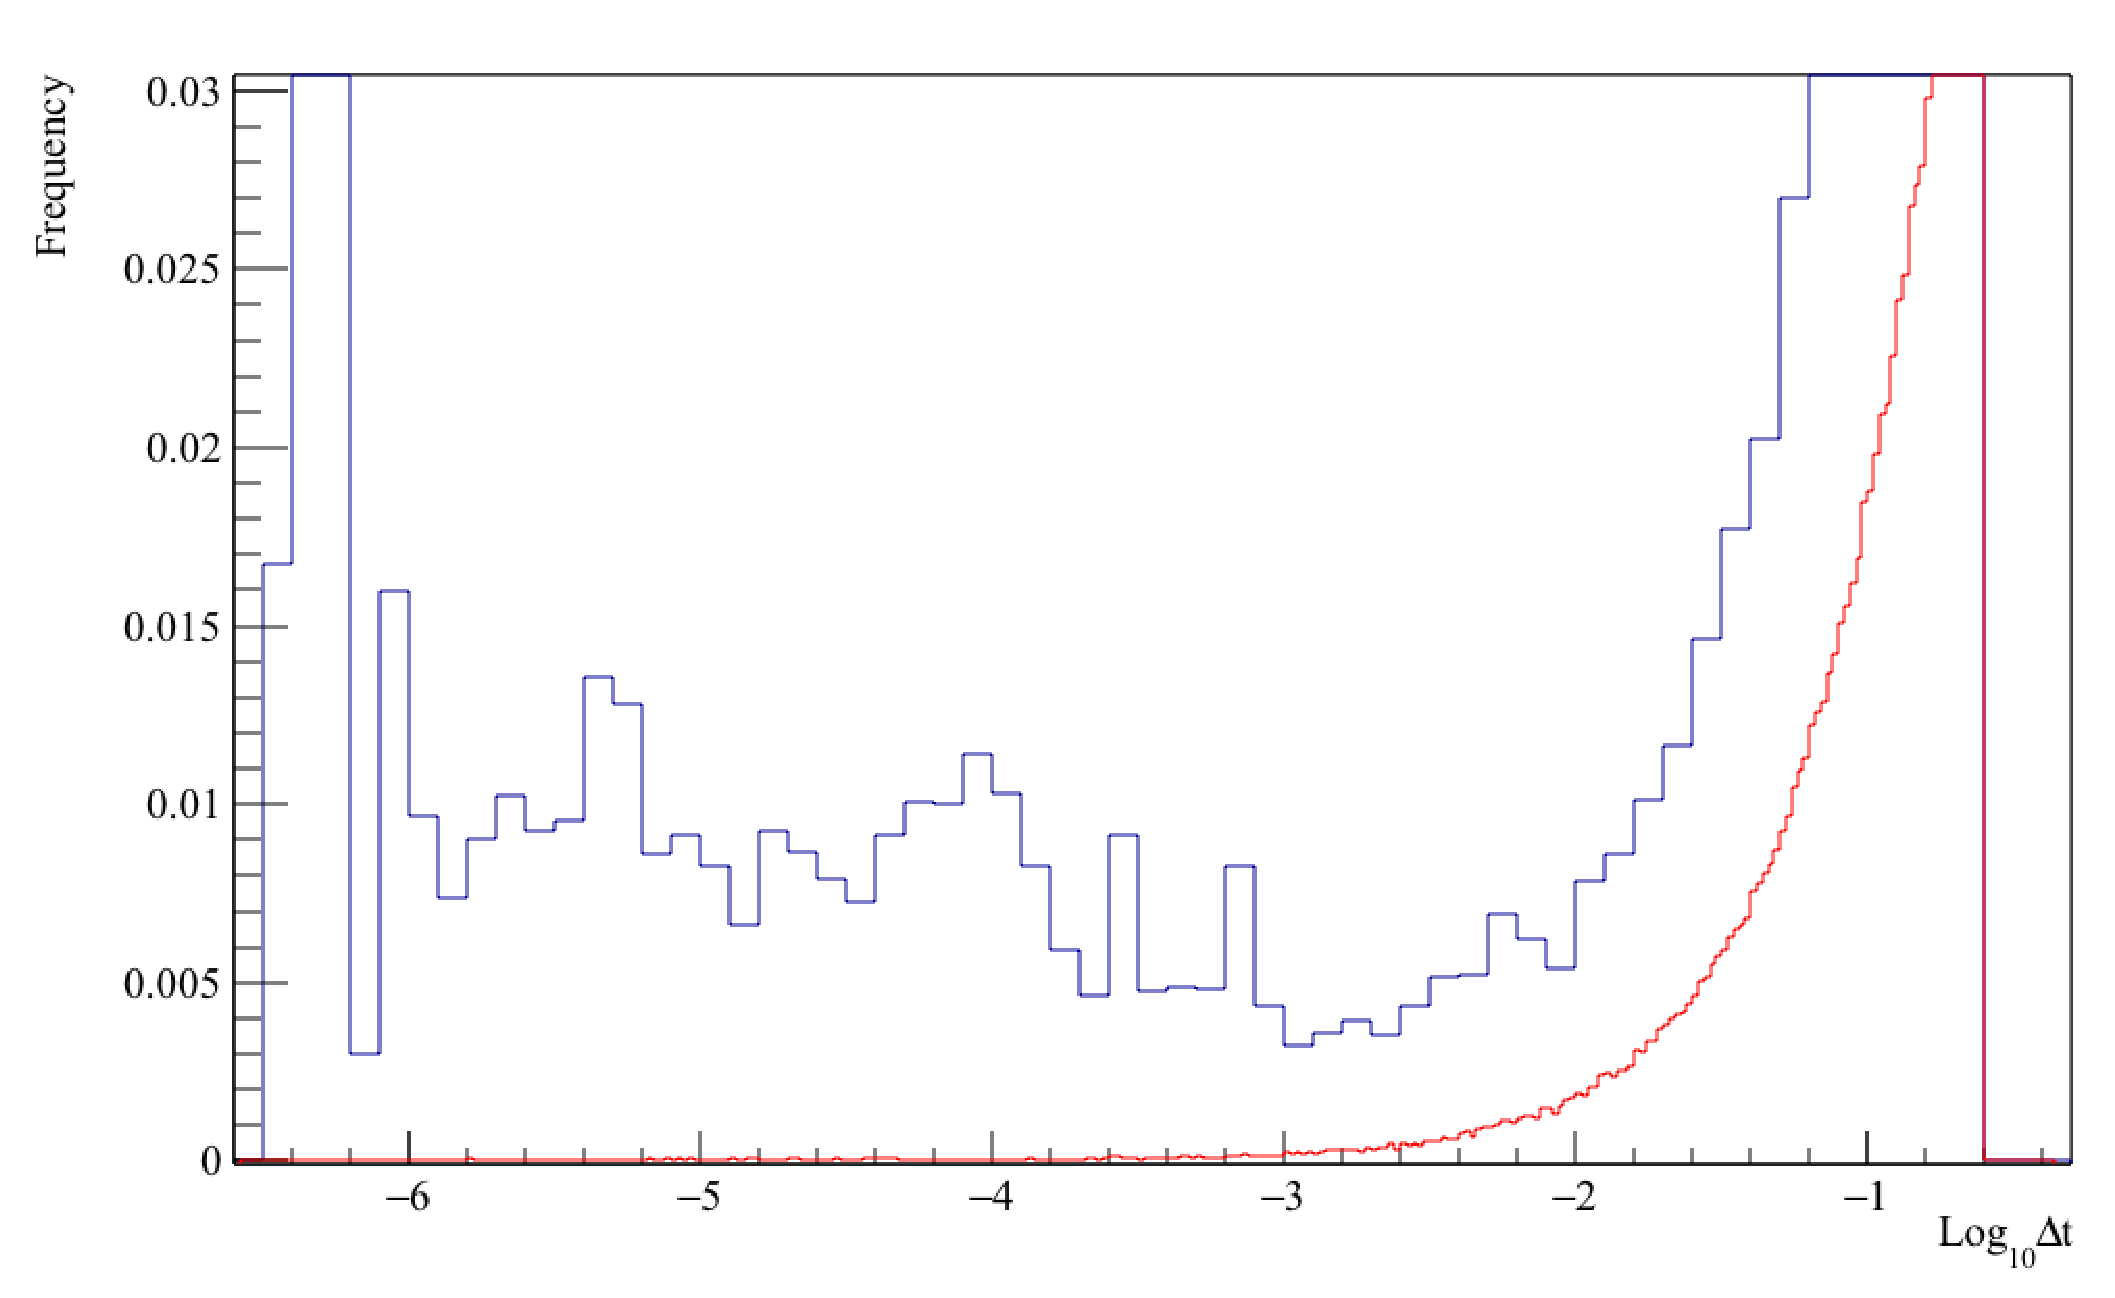
\includegraphics[width=0.74\textwidth]{mmf_pr_v_pf}
    \caption[Missed Muon Follower Example PDFs]{
        $P_R(N_2=20, \Delta t)$ (red) vs $P_F(N_1=60, N_2=20, \Delta t)$ (blue).}
\label{fig:mmf_sac}
\end{figure}
\begin{figure}[htbp]
    \centering
    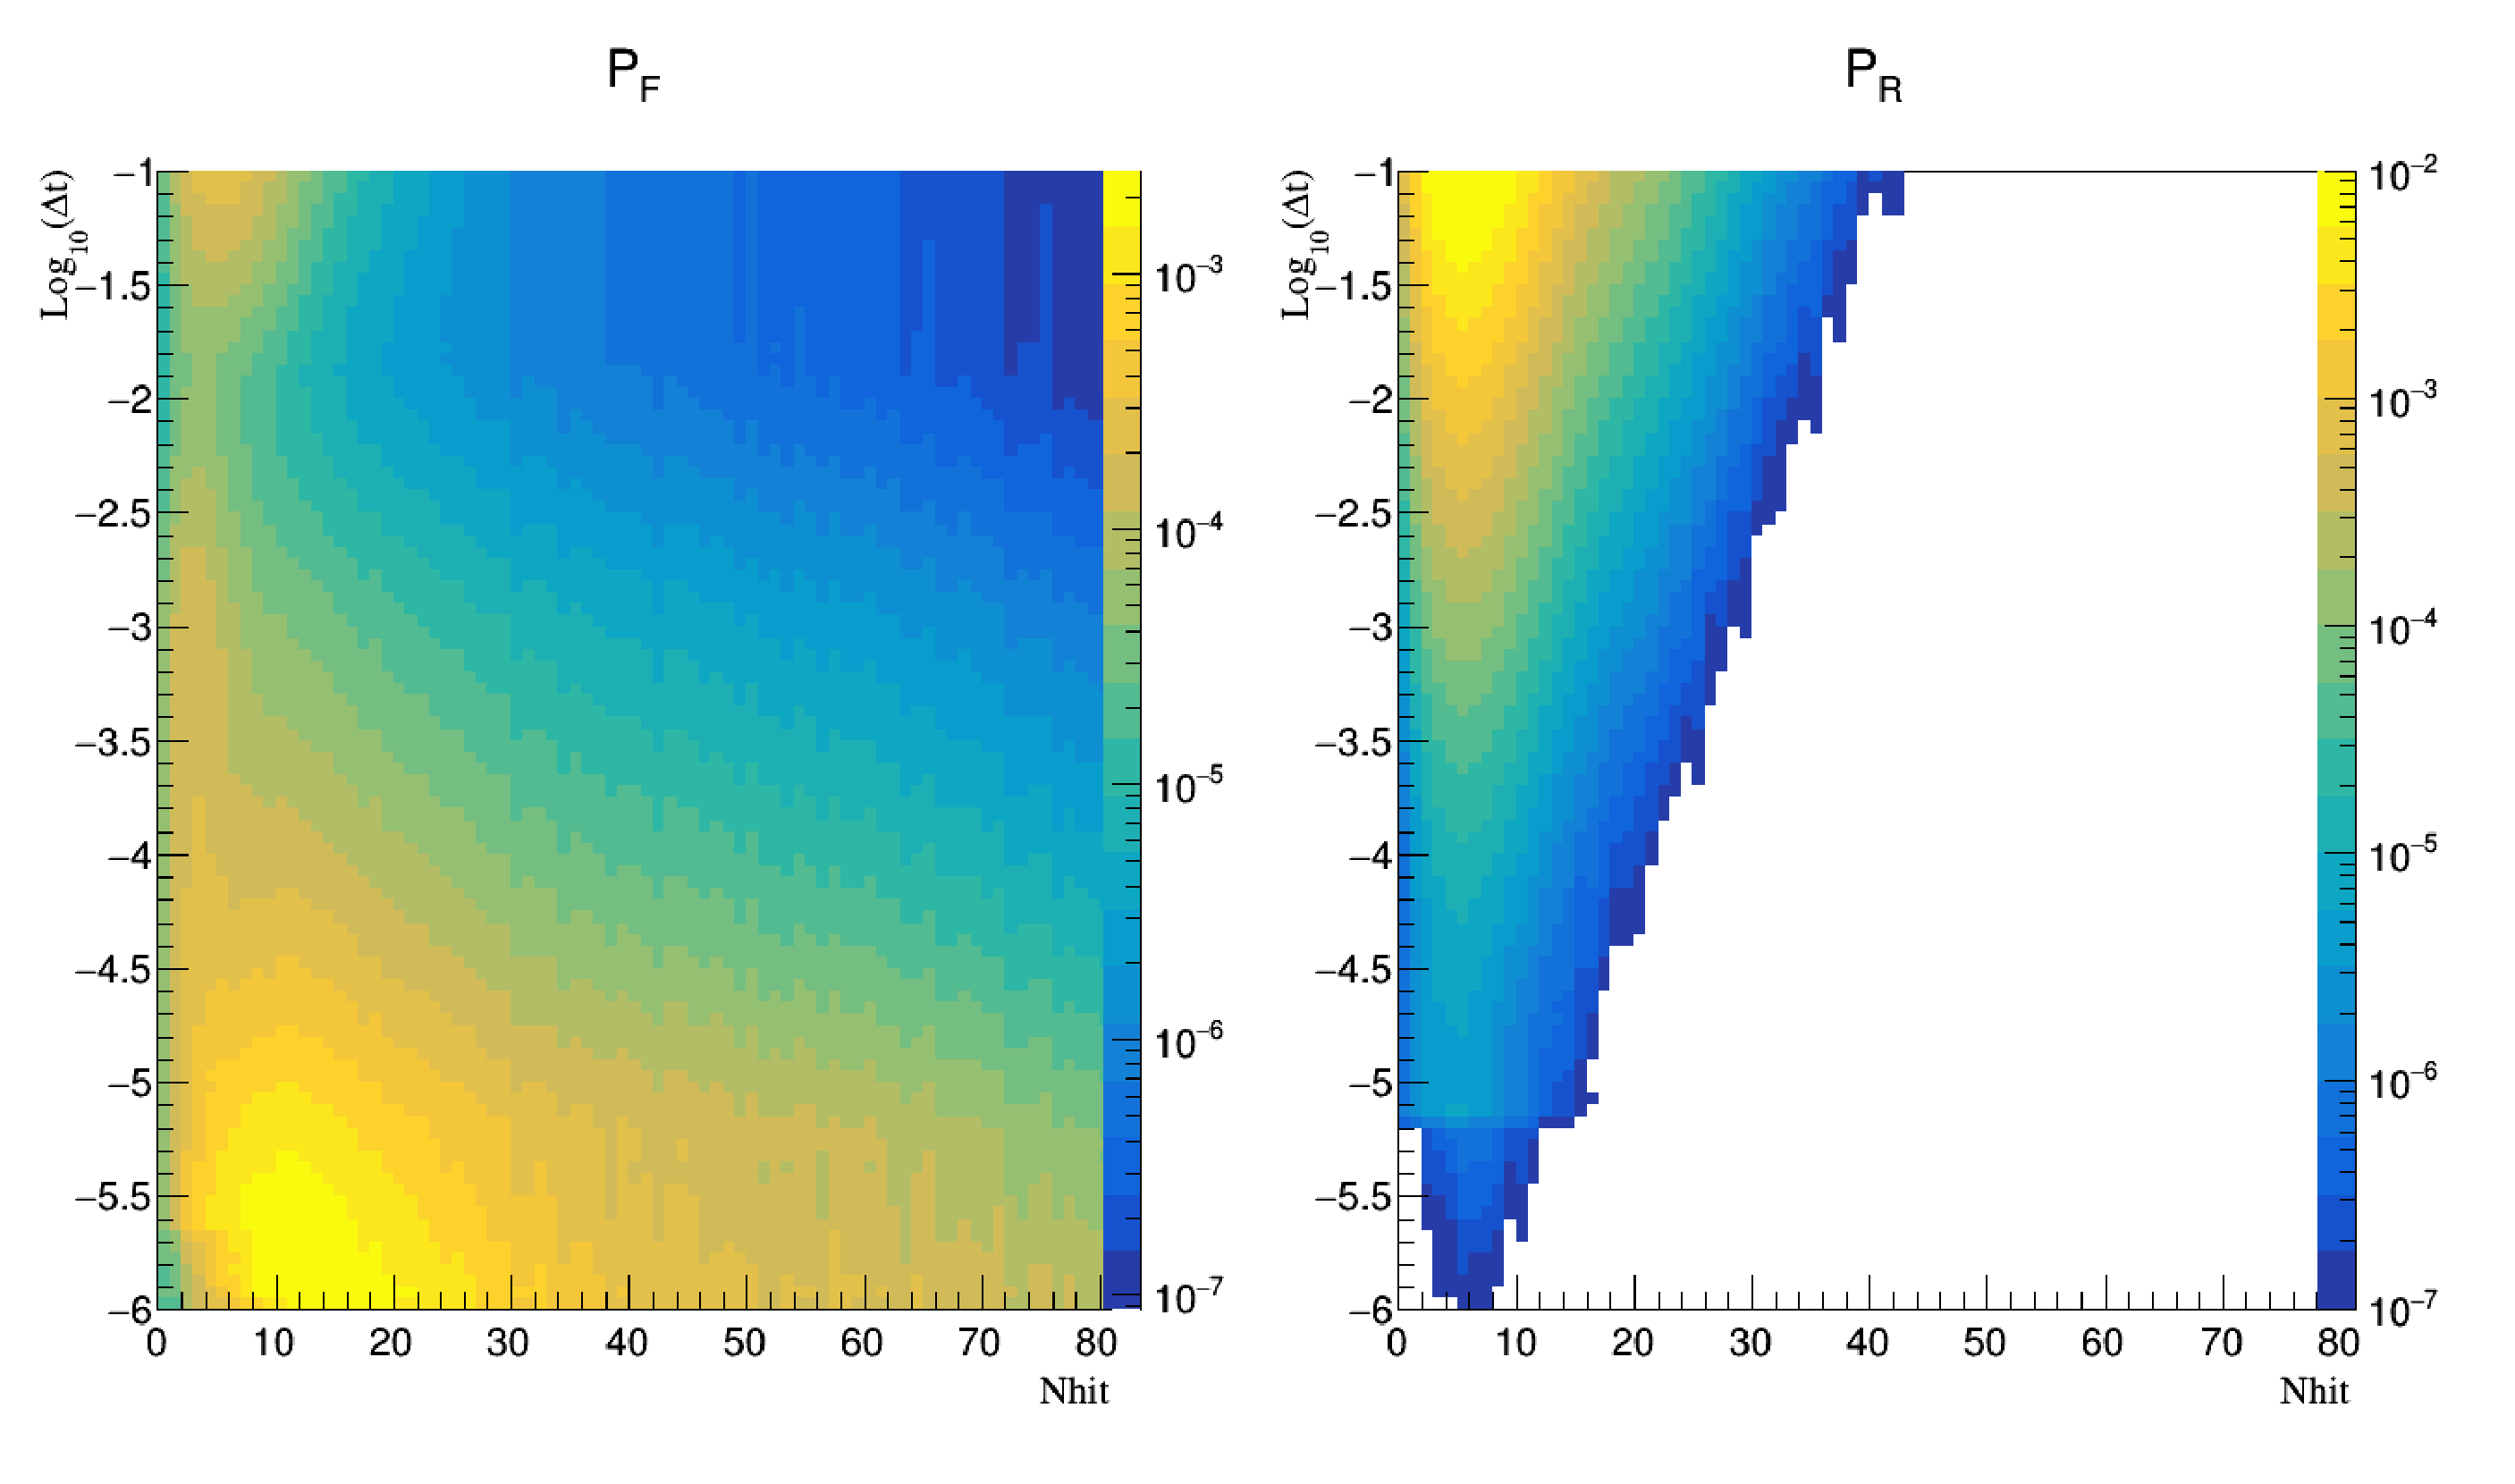
\includegraphics[width=0.74\textwidth]{mmf_bin_volume_normalized}
    \caption[Two-Dimensional Comparison for Missed Muon Follower]{
}
\label{fig:mmf_sac2}
\end{figure}
Figure~\ref{fig:mmf_sac} shows the measured distributions for $P_{F}$ and $P_{R}$
evaluated during the unblinded portion of the dataset;
a number of features exist in the observed distribution for $P_{F}$,
the peak at very short $\Delta t$ comes from re-triggers within the
detector following a high-nhit event.
Figure~\ref{fig:mmf_sac2} shows this comparison in two dimensions, each
bin along the Y-axis is normalized to account for the logarithmic change
in effective bin size.

Since there exists a number of selections from the threshold values of $N_{1}$,
$N_{2}$ and $\delta T$, the threshold value for $N_{1}$ was fixed at the SNO value
of $60$~\citep{neil_thesis}.
This value is motivated by the fact that time correlated events are more
likely to follow highly energetic events or events that can produce cosmogenic
isotopes, and the nhit threshold for these processes is not effected significantly
by the changes from SNO to SNO+.
The threshold value for $N_{2}$ was selected based upon what nhit of event
could possibly serve as a background to the solar or nucleon decay analysis,
a conservative value of $20$ was selected, which corresponds to an electron kinetic energy
of approximately $3$\,MeV.
With the two nhit constraints selected the $\delta t$ window was selected to
be as large as possible without incurring significant signal sacrifice,
the threshold value of $1$\,ms was selected.
From this a sacrifice of $0.01\%$ percent was determined~\citep{dc_document}.

\section{CAEN Cut}
I developed a new data cleaning cut, called the ``CAEN Cut'', that follows from
the AMB Cut from SNO\@.
The AMB Cut attempted to remove events from flashers the dataset by requiring
that the integral and peak height of the ESUMH trigger sum (as measured by the
AMB) fall below some threshold value.
The CAEN Cut performs a similar function, it calculates the baseline subtracted
integral and peak height of the digitized ESUMH trigger signal and places a cut on those values.

The baseline value of each trace is calculated as the average value of the first
$20$ samples and the $65^{\text{th}}$ to $85^{\text{th}}$ samples.
I chose to use two windows, one before the trigger pulse, one after the trigger pulse, to
correct for any overall slope across the digitized window.
The CAEN window is $104$ samples long, the final 19 samples are not used because they often
include a large noise pulse.
The noise pulse comes from the GT pulse arriving at the front-end and generating electrical noise,
it's typically called ``GT pickup''.
The noise makes the last $\approx20$ samples of the CAEN trace nearly
useless.

The determined baseline is subtracted from the CAEN trace and the integral and maximum
peak height are calculated from the samples between the two baseline windows.
To pass the CAEN Cut the peak and integral must fall between an upper and lower, nhit dependent,
cut cut value.
The cut values are given by
\begin{equation}
    f(n) = C\left(1-\sigma(n)\right) + \sigma(n)\left(mn+b\right)\text{.}
    \label{eqn:cc_threshold}
\end{equation}
Here $\sigma(x)$ indicates a sigmoid function,
\begin{equation}
    \sigma(x) = \frac{1}{1+e^{\frac{-(x-x_{0})}{w}}}
\end{equation}
The cut values are meant to be constant value at lower nhit, and then
linear with nhit above $\approx15$ nhit, the sigmoid allows for a smooth
transition between those two functions; for both the upper and lower threshold
the sigmoid position ($x_{0}$) and width ($w$) are $15$\,nhit and $5$\,nhit respectively.
The constant value at lower nhit is $C$ the slope of the line at higher nhit
is given by $m$ and the value $b$ is required to be
\begin{equation}
    b = \frac{C}{mx_{0}}
\end{equation}
so that there is not discontinuity between the two cut regions.
\begin{table}
    \centering
  \begin{tabular}{c | c c}
      & Constant & Slope  \\
      \hline
      Upper Bound & 658.8 & -6.61\\
      Lower Bound & -707.0 & -15.9\\
    \end{tabular}
    \caption[CAEN Cut Values]{The upper and lower bounds for the CAEN Cut as
    described in Eqn.~\eqref{eqn:cc_threshold}.
    Constant values are in ADC Counts, slope values are ADC Counts per nhit.}
\label{tbl:caen_cut}
\end{table}
The values for these parameters are given in Table~\ref{tbl:caen_cut}.

The reason for the two cut regions is because at lower nhit the signal
peak is smaller than the noise one the ESUMH signal, so the only requirement
is that the peak and integral be consistent with a noise only trigger sum.
At higher nhit the ESUMH signal scales linearly with nhit, each new hit
adds approximately the same amount of height to the trigger pulse.

The cut parameters were determined from two calibration datasets, the first was
tagged $\ce{^{16}N}$
events. The second was a sample of $PULSE\_GT$ triggers taken during normal
running.
The two datasets are used to determine the cut parameters for the two
different cut regions.
The $\ce{^{16}N}$ data was used to determine cut values for the higher nhit
region, the $PULSE\_GT$ data was used for the lower nhit cut values.

\begin{figure}[htbp]
    \centering
    \begin{subfigure}[b]{0.48\textwidth}
        \centering
        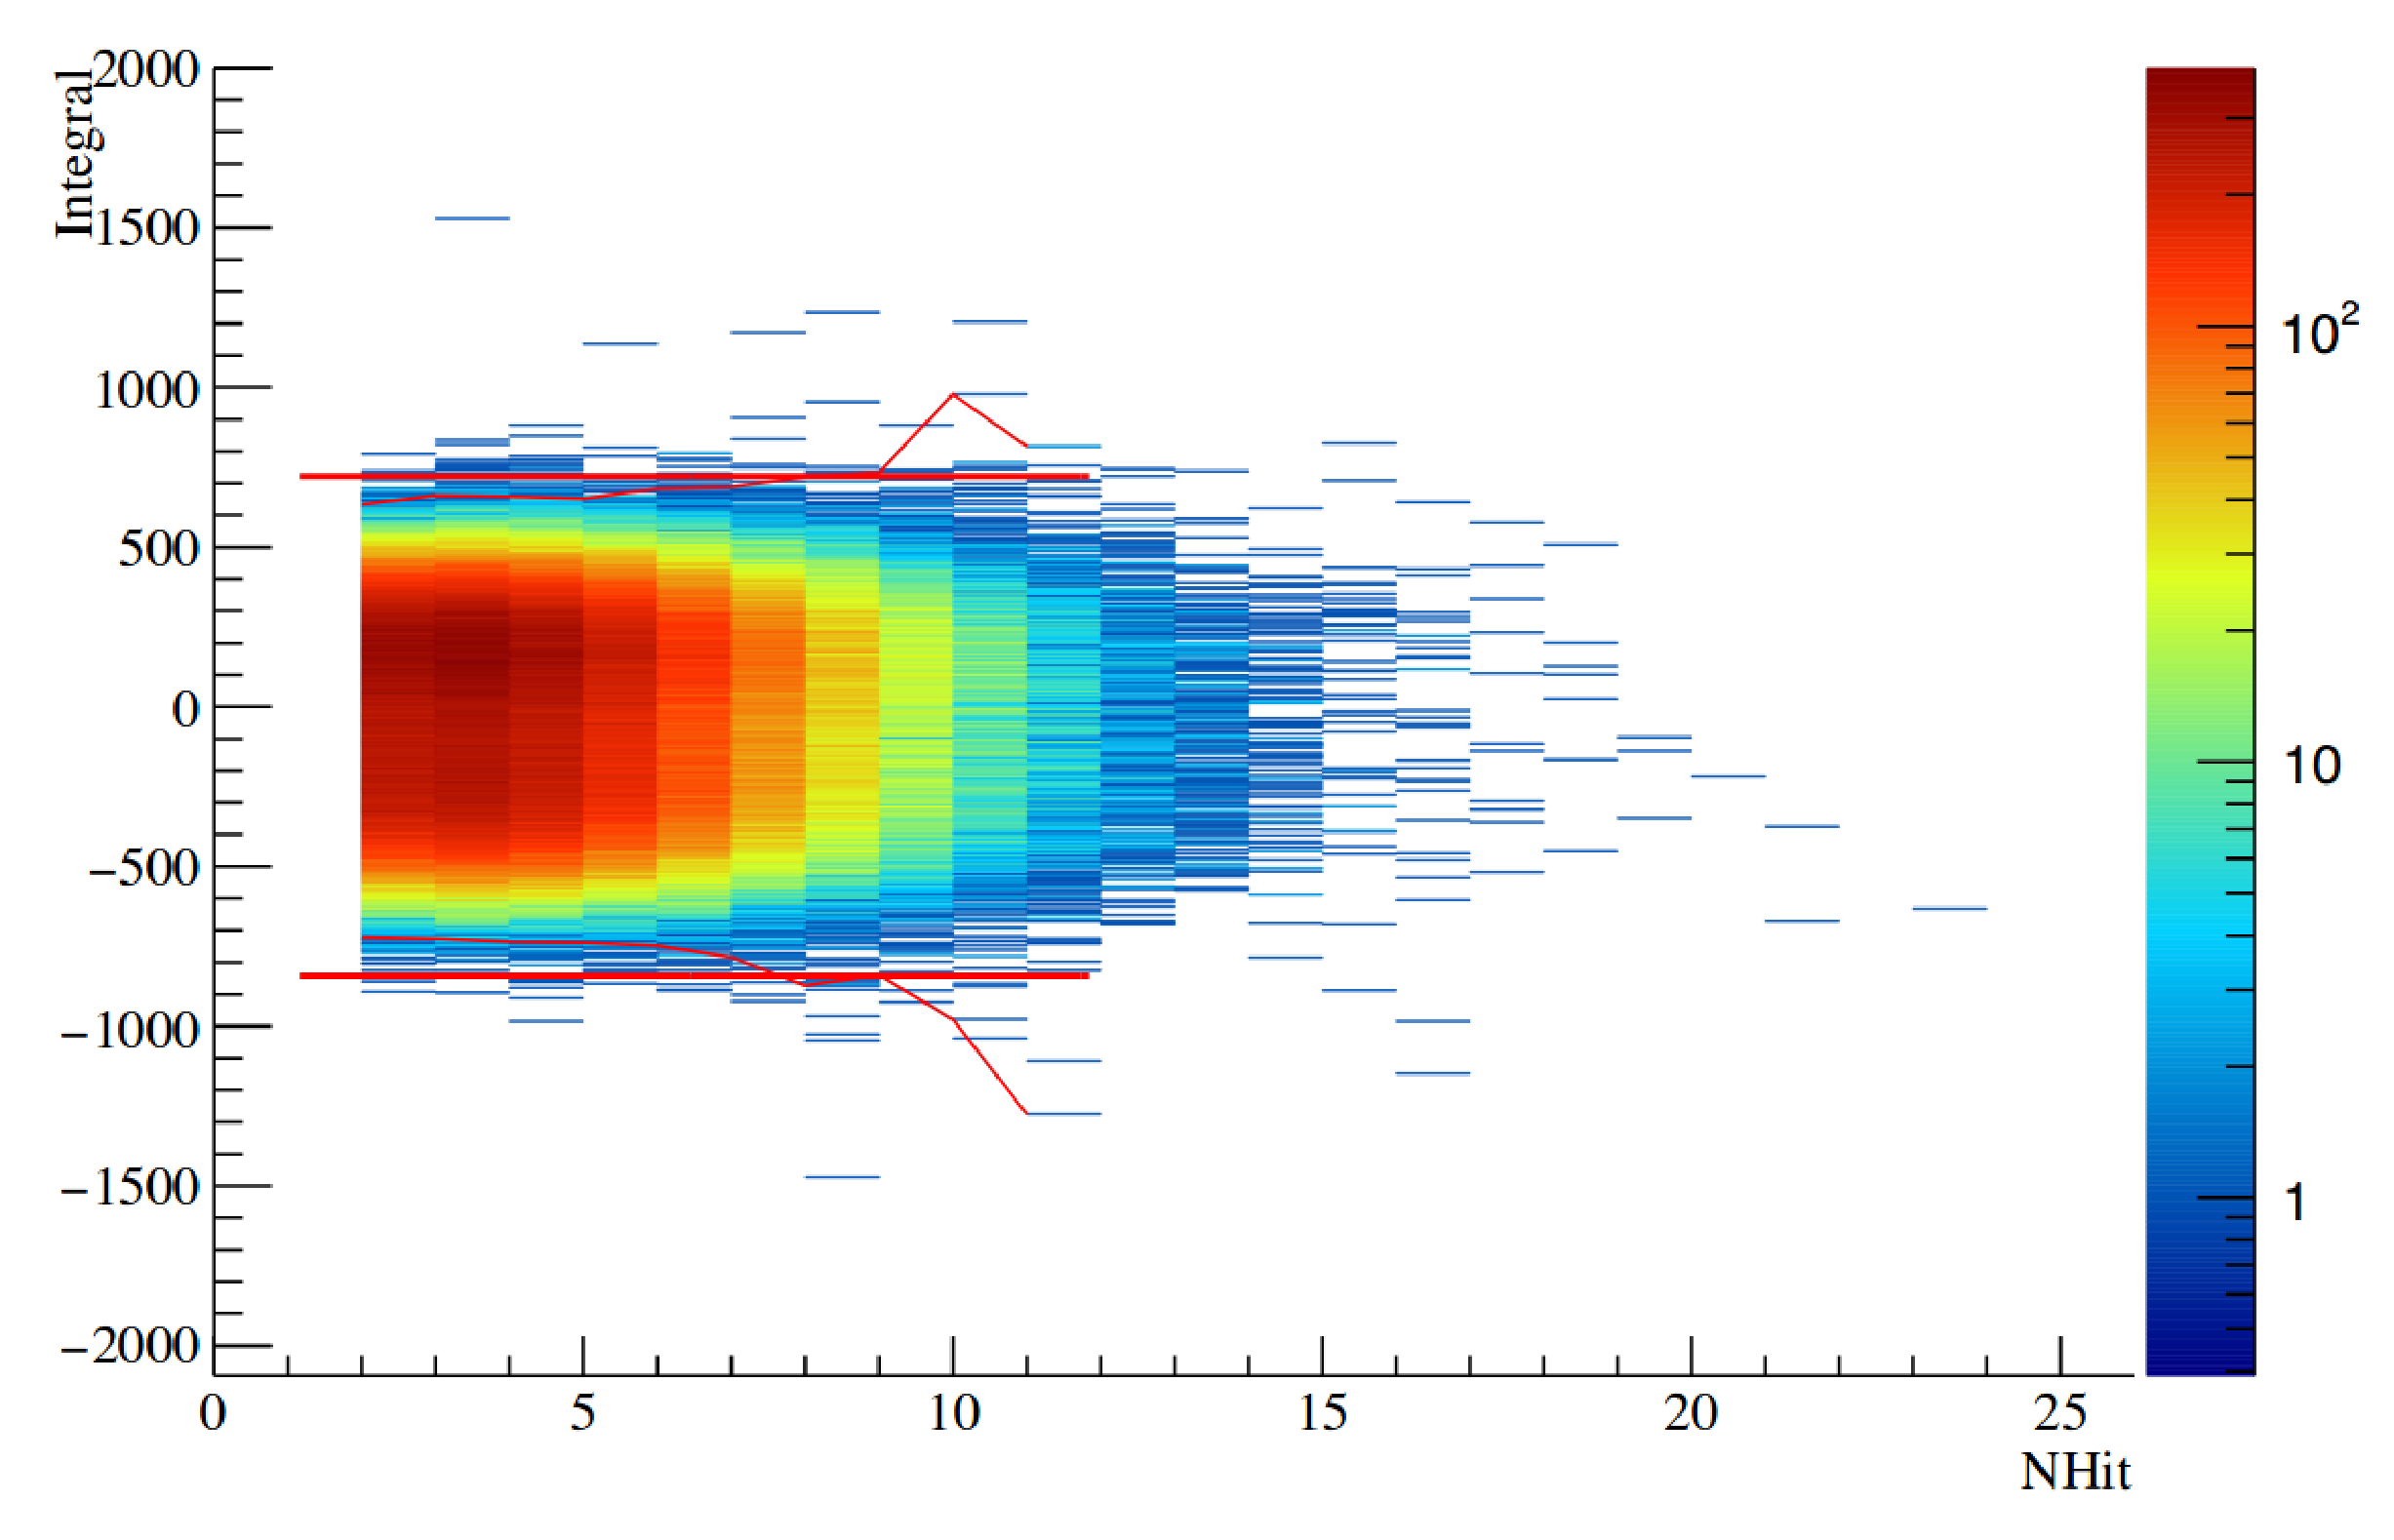
\includegraphics[width=\textwidth]{caen_pgt}
        \caption[]{}
    \end{subfigure}
    \hfill
    \begin{subfigure}[b]{0.48\textwidth}
        \centering
        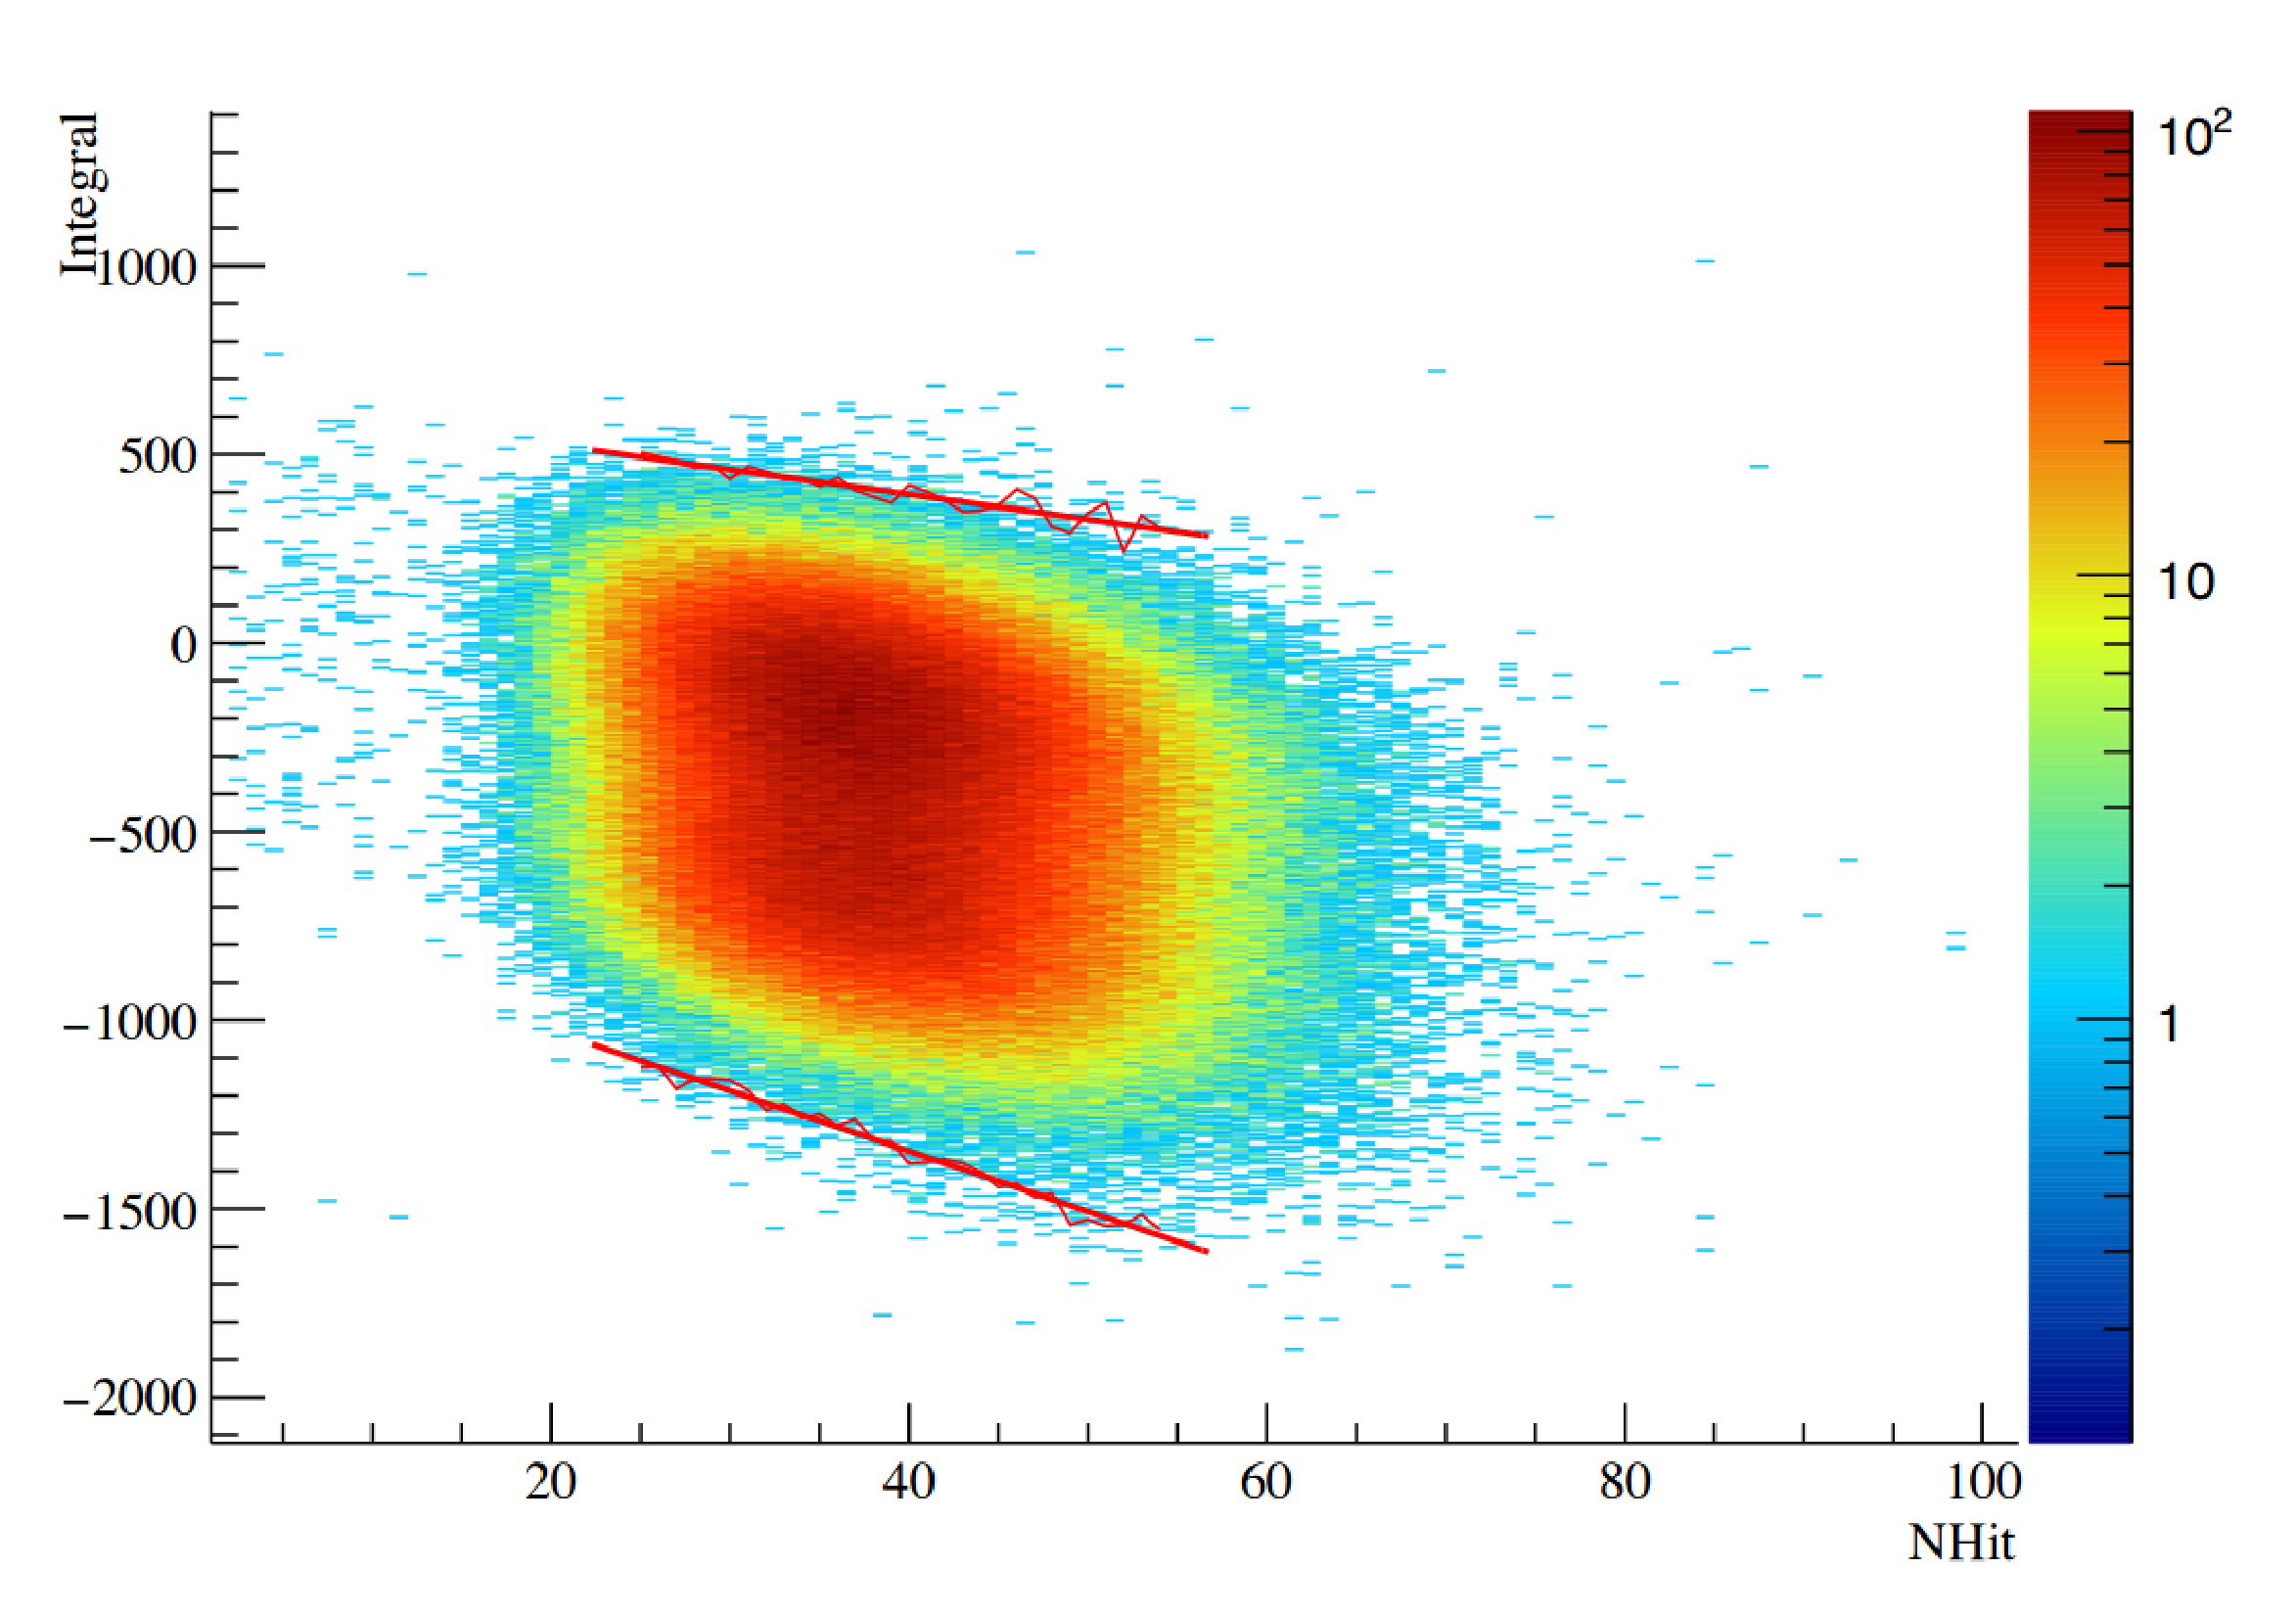
\includegraphics[width=\textwidth]{caen_n16}
        \caption[]{}
    \end{subfigure}

    \begin{subfigure}[b]{0.50\textwidth}
        \centering
        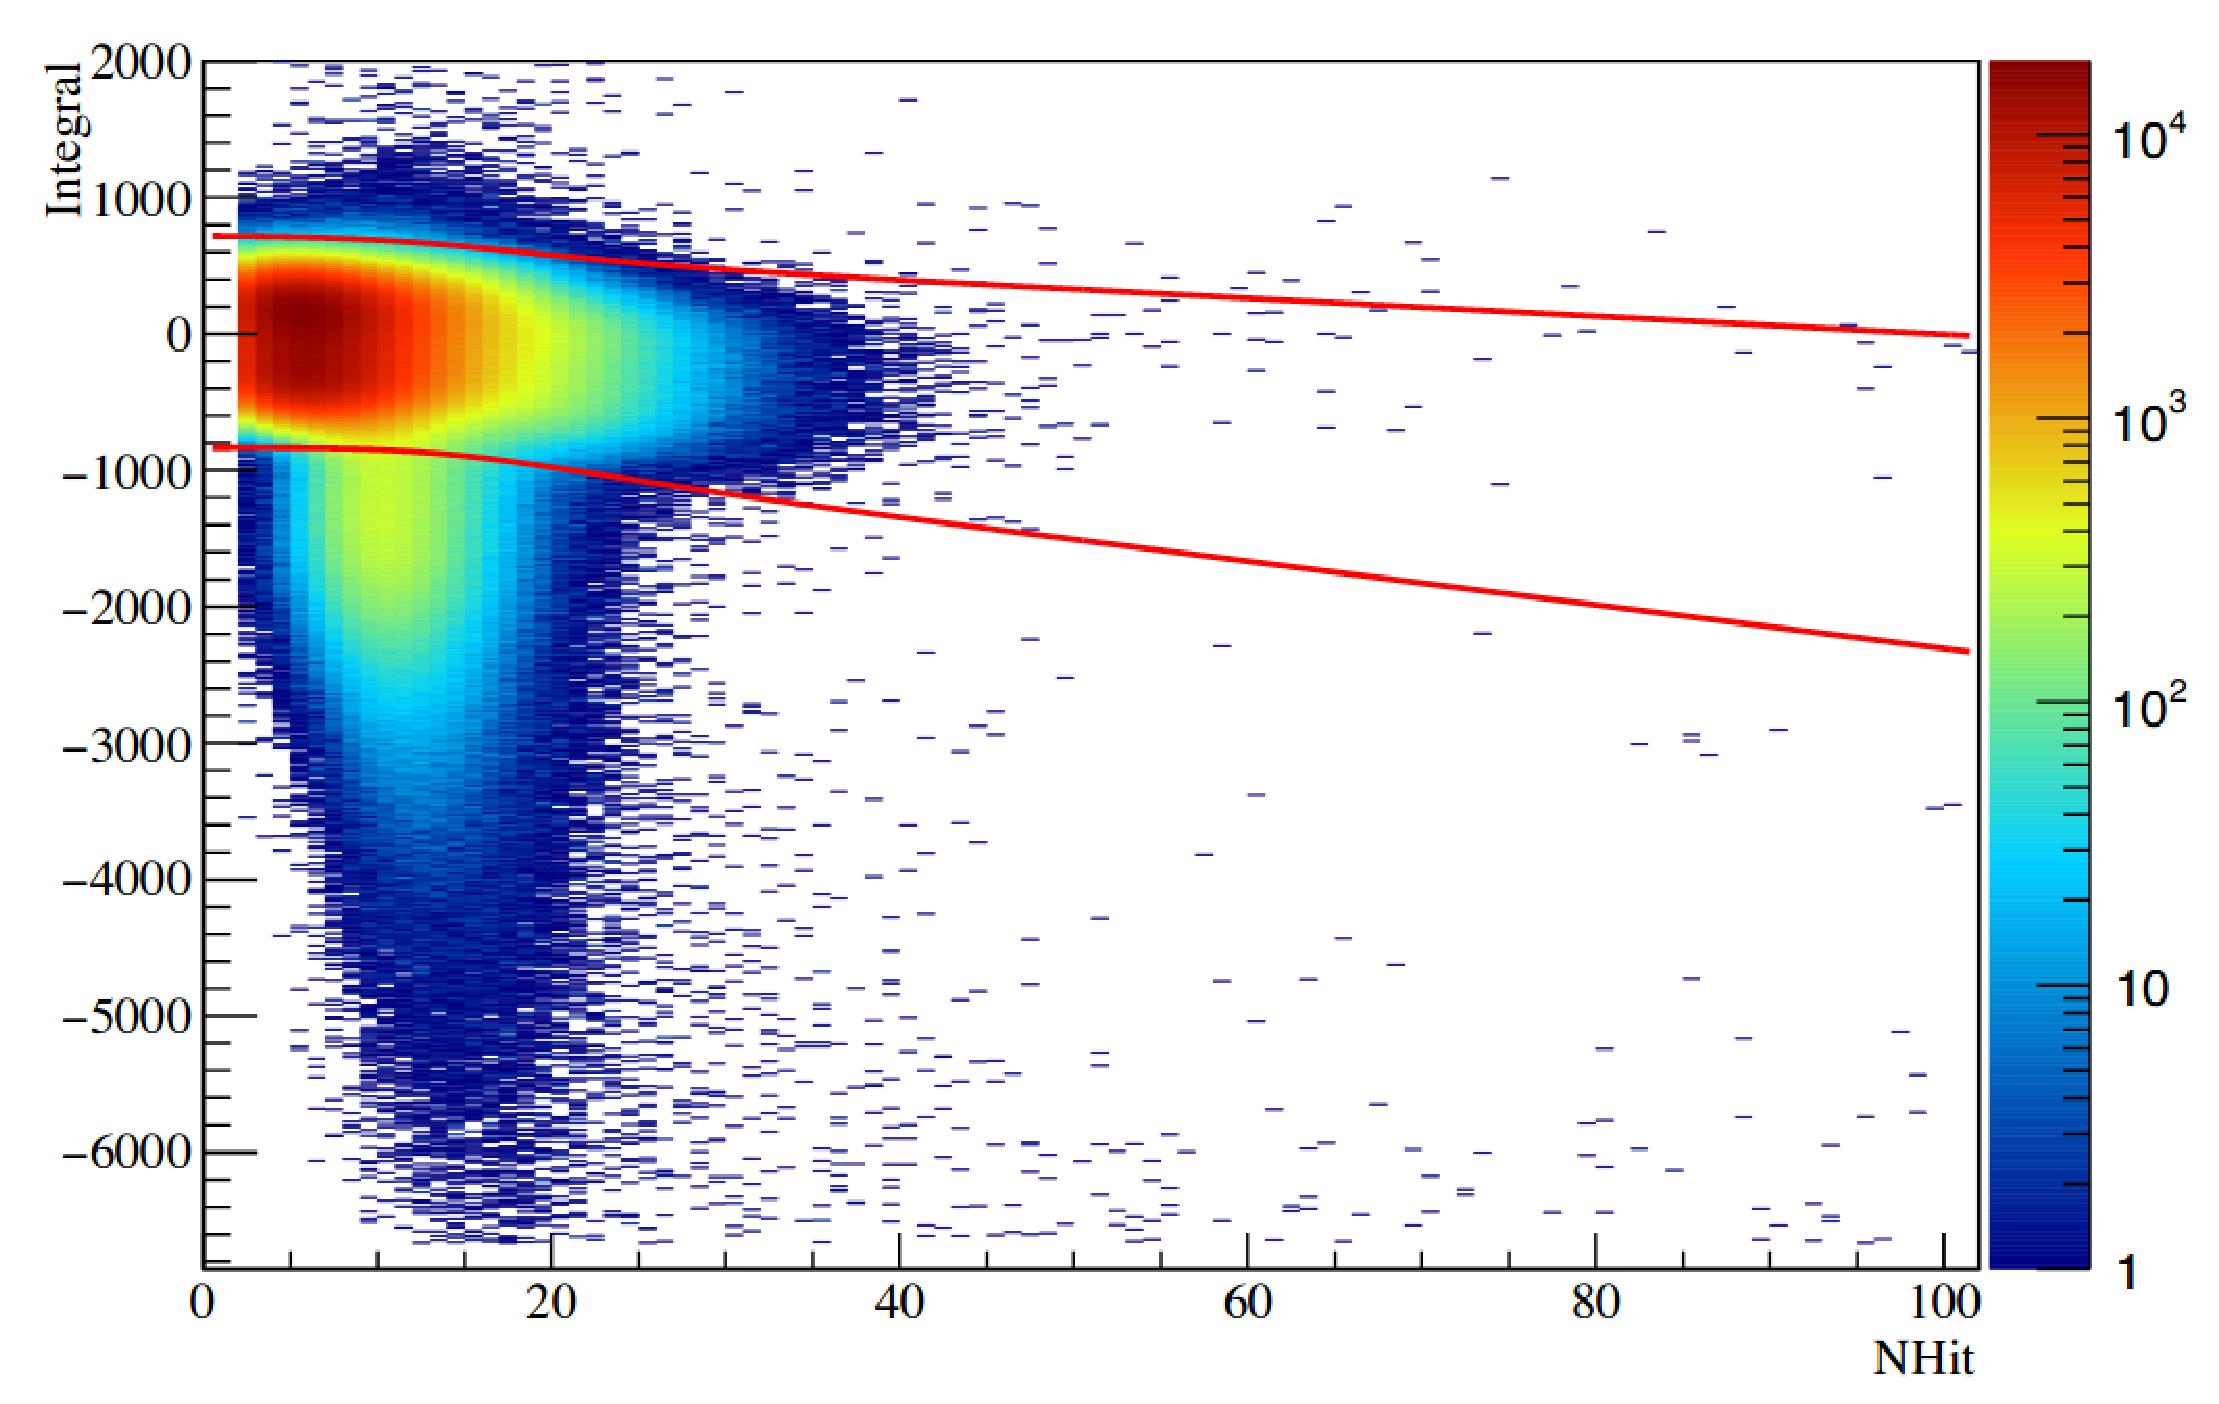
\includegraphics[width=\textwidth]{caen_physics}
        \caption[]{}
    \end{subfigure}
    \caption[]{Distribution of CAEN integral for $PULSE\_GT$ (a), $\ce{^{16}N}$ (b), and
    standard physics triggered (c) events. Integral values are in ADC counts
    and Z-axis values are counts. The thin red lines indicate the 99\% inclusion
    values and the thick red lines indicate the best fit functions.}
    \label{fig:caen_inclusion}
\end{figure}

For both regions the value of the integral or peak height that include
99\% of the events at each nhit is found. Then the parameters of
Eqn.~\ref{eqn:cc_threshold} that best fit those points is determined.
Then Eqn.~\ref{eqn:cc_threshold} with the best fit upper and lower
parameters to include 99\% of the calibration data become the threshold
values for rejecting flasher events.
The 99\% criteria was chosen arbitrarily to ensure that the fraction of
``good'' events rejected by this cut was similar to that of other data
cleaning cuts.
Figure~\ref{fig:caen_inclusion} shows how the ESUMH CAEN trace integral is distributed
in the two calibration datasets and for standard physics data taking.



%TODO move this shit to an appendix
%\subsection{ZeroZero Cut}
%The GTID for the FEC is stored in a ripple counter, it's often the case that
%when the bottom two bits of the counter rollover the event that gets recorded in
%the FEC memory gets corrupted.
%When this happens the builder cannot put the corrupted hits into the event correctly,
%and the hits will effectively be discarded.
%This means that event the detectors effective photon detection efficiency is lower
%for events that have a GTID with $00$ in the bottom two bits.
%Rather than correct for this inefficiecy in reconstruction, events with GTID
%ending in $00$ are discarded. This corresponds to a random pre-scale
%on our by a factor of $\frac{1}{256}$.
%\subsection{Crate Isotropy Cut}
%The Crate Isotropy Cut is designed to remove events that are isolated
%in one or a few electronics crates.
%Events originating from light within the detector are unlikely to have any
%preference in electronics space.
%However hits caused by electrical noise that was created near the electronics
%can show a very distinct preference for one crate.
%The criteria for this cut is that fraction of hits in any single
%is greater that $70\%$ and that the fractions of hits within
%that crate are either $80\%$ within adjacent FECs or $70\%$ within
%adjacent channels.
%%\subsection{Flasher Geometry Cut}
%%\subsection{ITC Timespread Cut}

%\chapter{Another Appendix}
\end{appendices}
